\documentclass{article}

\usepackage{graphicx}
\usepackage{tikz}
\usepackage{tikzsymbols}
\usetikzlibrary{calc,patterns,shapes.geometric}
\pagestyle{empty}
\usepackage[margin=0pt]{geometry}
\geometry{papersize={14in,12in}}

\def\centerarc[#1](#2)(#3:#4:#5){\draw[#1] ($(#2)+({#5*cos(#3)},{#5*sin(#3)})$) arc (#3:#4:#5);}

\begin{document}
	\begin{figure}
		\centering
		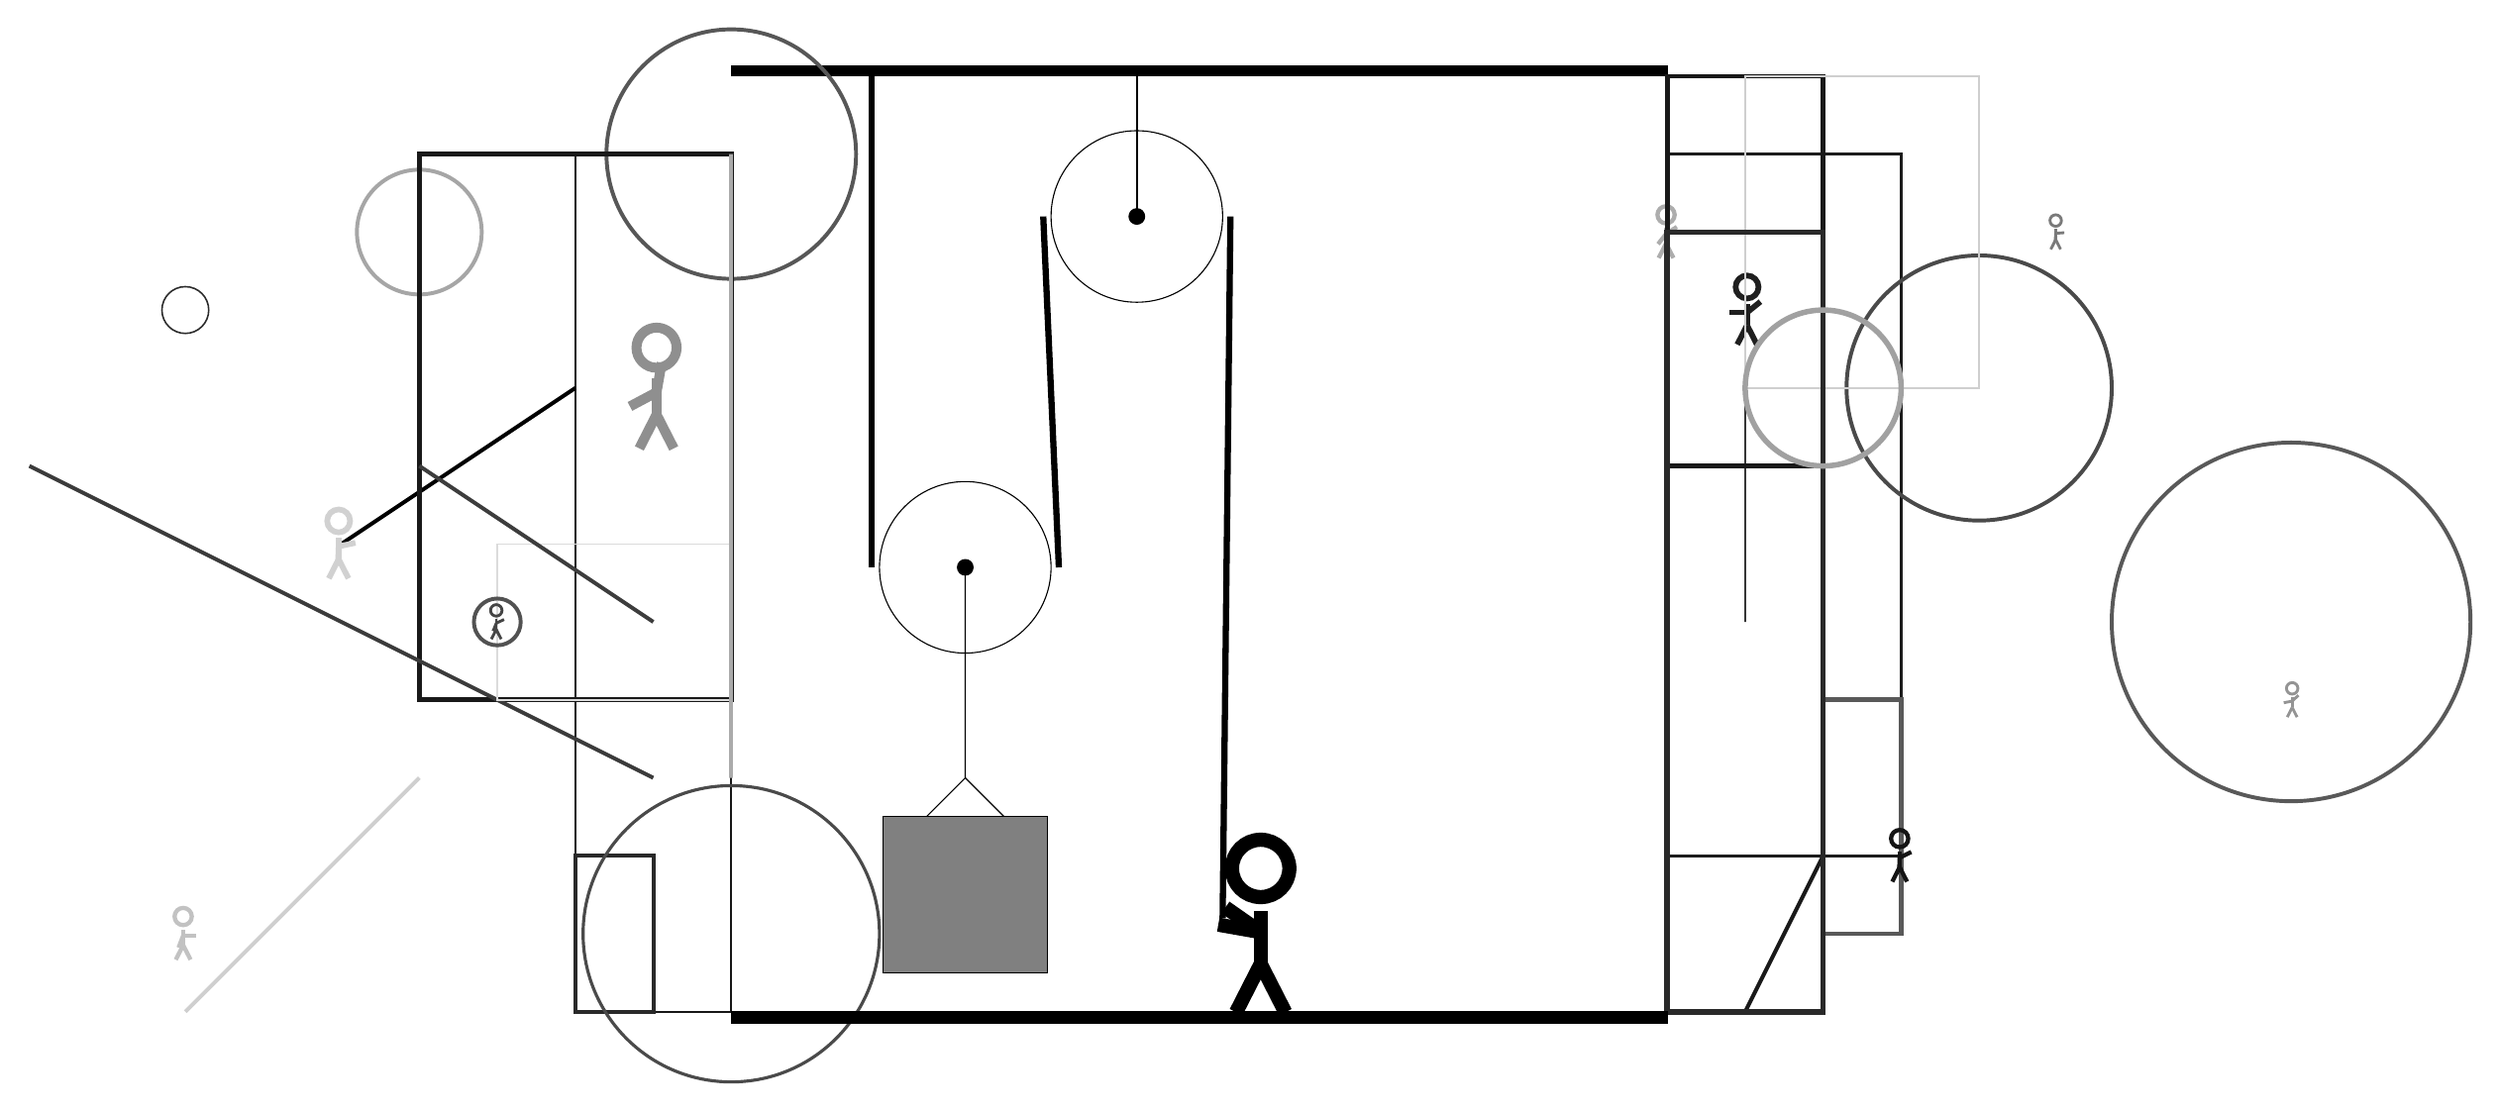
\begin{tikzpicture}
			%%%%% START %%%%%
			
			\draw[fill=black] (-2, 9) rectangle (10, 9.125);
			
			\draw (3.2, 7.2) circle (1.1);
			\draw[fill=black] (3.2, 7.2) circle (0.1);
			\draw[thick] (3.2, 7.2) -- (3.2, 9);
			
			\draw (1, 2.7) circle (1.1);
			\draw[fill=black] (1, 2.7) circle (0.1);
			
			\draw (1, 2.7) -- (1, 0) -- (0.5, -0.5);
			\draw (1, 0) -- (1.5, -0.5);
			\draw[fill=black!50] (-0.05, -0.5) rectangle (2.05, -2.5);
			
			\draw[line width=0.8mm] (-0.2, 9) -- (-0.2, 2.7);
			\centerarc[line width=0.8mm](1, 2.7)(180:360:1.2000000000000002);
			\draw[line width=0.8mm](2.2, 2.7) -- (2.0, 7.2);
			\centerarc[line width=0.8mm](3.2, 7.2)(0:180:1.2000000000000002);
			\draw[line width=0.8mm](4.4, 7.2) -- (4.3, -1.8);
			
			\node at (4.7, -1.9) {\Strichmaxerl[10][-35][170]};
			
			\draw[line width=0.3mm, color=black!79] (11, 5) rectangle (11, 2);
			
			\draw[line width=0.4mm, color=black!89] (10, -1) rectangle (13, 8);
			\node[line width=0.5mm, color=black!42] at (18, 1) {\Strichmaxerl[2][11][43]};
			\node[line width=0.7mm, color=black!88] at (11, 6) {\Strichmaxerl[4][0][39]};
			\node[line width=0.2mm, color=black!32] at (10, 7) {\Strichmaxerl[3][52][33]};
			
			\draw[line width=0.5mm, color=black!19](-6, 0) -- (-9, -3);
			\draw[line width=0.3mm, color=black!91] (-2, -3) rectangle (-4, 8);
			\draw [line width=0.5mm, color=black!71](14, 5) circle (1.7);
			\node[line width=0.5mm, color=black!52] at (15, 7) {\Strichmaxerl[2][86][4]};
			\draw [line width=0.5mm, color=black!66](-2, 8) circle (1.6);
			\draw [line width=0.5mm, color=black!35](-6, 7) circle (0.8);
			\draw[line width=0.5mm, color=black!100](-7, 3) -- (-4, 5);
			\draw[line width=0.6mm, color=black!65] (12, 1) rectangle (13, -2);
			
			\draw[line width=0.6mm, color=black!90] (-2, 1) rectangle (-6, 8);
			\draw[line width=0.5mm, color=black!77](-3, 0) -- (-11, 4);
			\draw[line width=0.2mm, color=black!14] (-2, 3) rectangle (-5, 1);
			
			\draw[line width=0.5mm, color=black!90](11, -3) -- (12, -1);
			\node[line width=0.7mm, color=black!92] at (13, -1) {\Strichmaxerl[3][88][26]};
			\node[line width=0.7mm, color=black!44] at (-3, 5) {\Strichmaxerl[7][28][80]};
			\draw[line width=0.5mm, color=black!76](-6, 4) -- (-3, 2);
			\node[line width=0.2mm, color=black!24] at (-9, -2) {\Strichmaxerl[3][69][0]};
			
			\draw[line width=0.5mm, color=black!84] (-4, -3) rectangle (-3, -1);
			
			\draw[line width=0.6mm, color=black!90] (12, 4) rectangle (10, 9);
			\node[line width=0.2mm, color=black!73] at (-5, 2) {\Strichmaxerl[2][68][25]};
			\draw[line width=0.5mm, color=black!75](12, 7) -- (12, 5);
			\draw [line width=0.5mm, color=black!68](-5, 2) circle (0.3);
			\draw [line width=0.2mm, color=black!83](-9, 6) circle (0.3);
			\draw[line width=0.2mm, color=black!19] (11, 5) rectangle (14, 9);
			\node[line width=0.2mm, color=black!18] at (-7, 3) {\Strichmaxerl[4][88][12]};
			\draw [line width=0.4mm, color=black!71](-2, -2) circle (1.9);
			\draw [line width=0.5mm, color=black!65](18, 2) circle (2.3);
			
			\draw[line width=0.5mm, color=black!33] (-2, 8) rectangle (-2, 0);
			\draw[line width=0.3mm, color=black!43] (12, 3) rectangle (12, -3);
			\draw[line width=0.7mm, color=black!84] (10, 7) rectangle (12, -3);
			\draw [line width=0.7mm, color=black!37](12, 5) circle (1.0);
			
			\draw[fill=black] (-2, -3) rectangle (10, -3.15);
			
			%%%%% END %%%%%
		\end{tikzpicture}
	\end{figure}	
\end{document}